% !TEX root = MutationTestingSurvey.tex

\section{Mutation Testing Process}
\label{sec:process}

	\begin{figure}
	\centering
		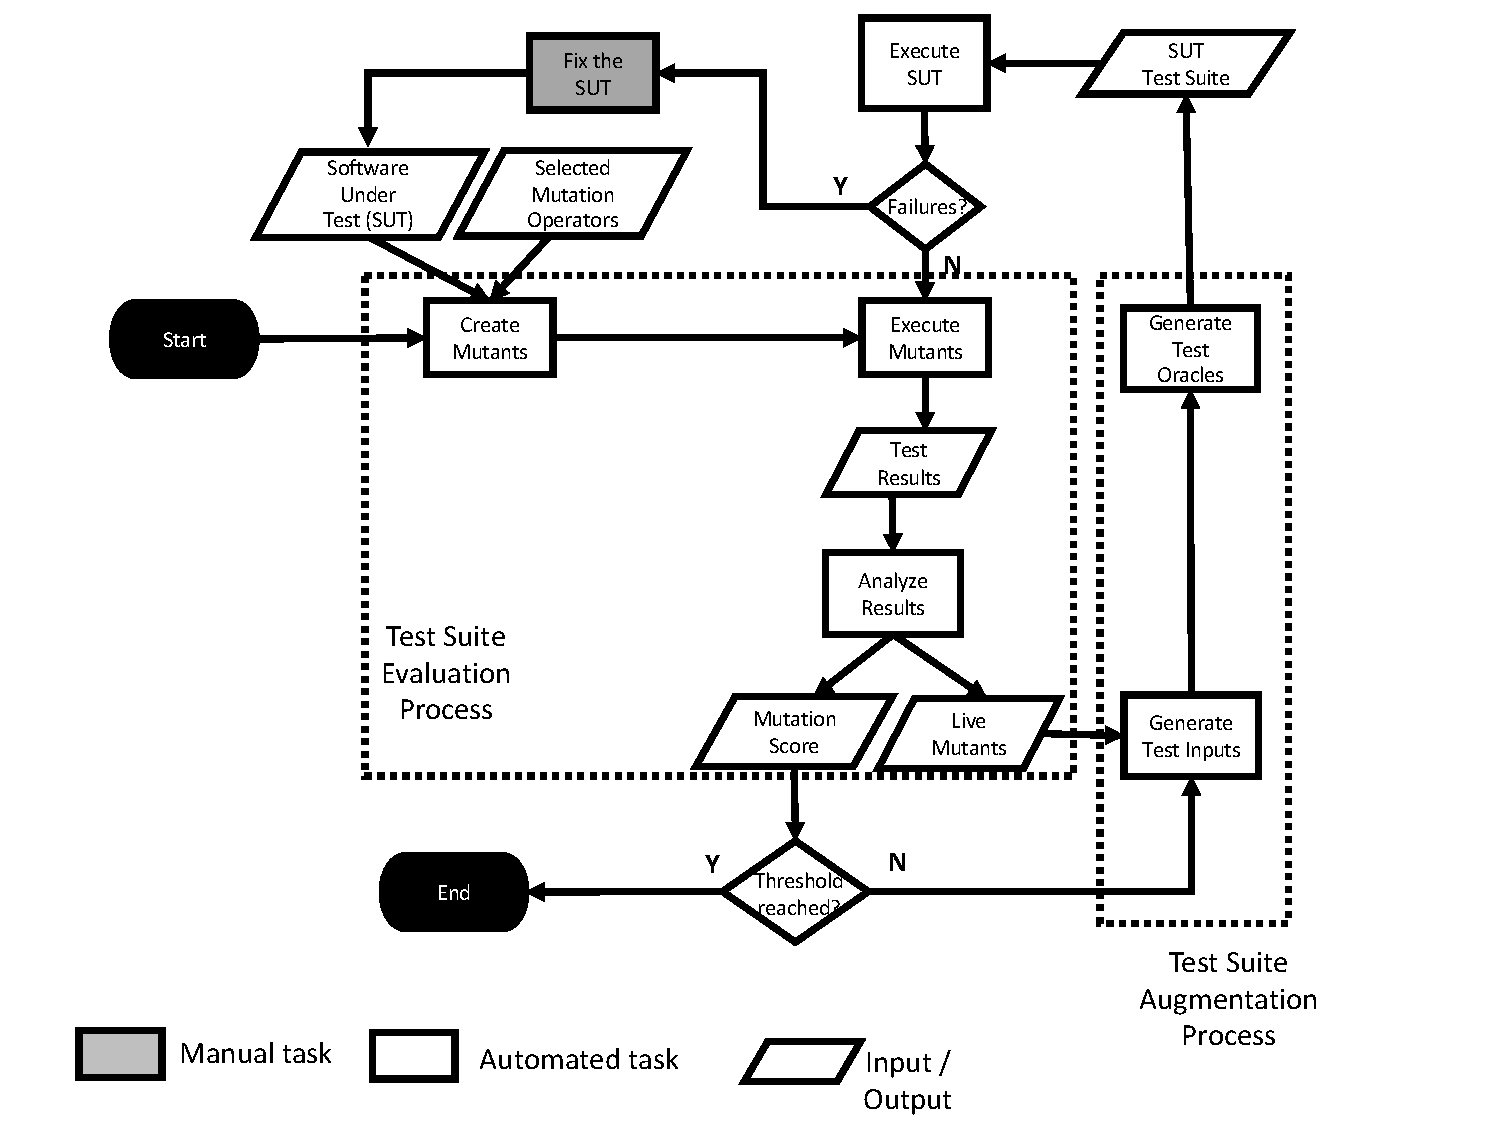
\includegraphics[width=\textwidth]{images/process}
		\caption{Mutation Testing Process.}
		\label{fig:code:process}
	\end{figure}

Figure \ref{fig:code:process} shows the reference code-driven mutation testing process that will be considered in this book. The process depicted in Figure \ref{fig:code:process} has been inspired by the mutation testing process described in related work \cite{offutt2001mutation,papadakis2019mutation}. The process is based on two main sub-processes, \emph{Test Suite Evaluation} and \emph{Test Suite Augmentation}. Sections~\ref{sub:test_suite_evaluation} and  provide an overview of each of them, Sections~\ref{sub:test_suite_evaluation}~to~\ref{sub:test_suite_augmentation} describe in details the building blocks and the issues to overcome in order to efficiently apply code oriented data mutation.

\subsection{Test Suite Evaluation} % (fold)
\label{sub:test_suite_evaluation}

The Test Suite Evaluation process concerns the automatic generation of modified versions (i.e., the mutants) of the software under test (SUT) and the evaluation of the quality of the SUT test suite. It consists of three activities: \emph{create mutants}, \emph{execute mutants}, and \emph{analyze results}. 
These activities are typically automated by toolsets that often include strategies to address scalability issues. Mutation testing activities and related optimizations are depicted in Figure~\ref{fig:code:process} and described in the following paragraphs.

The Test Suite Evaluation process starts with engineers providing the SUT and a selection of the mutation operators to consider. The set of mutation of available mutation operators typically depends on the toolset implementing the mutation testing process. 
A typical set of mutation operators implemented by most of the existing toolsets consists of the relational (ROR), logical (LCR), arithmetic (AOR), absolute (ABS) and unary insertion (UOI) operators \cite{rothermel1996experimental}. 
%Several research paper target the definition of mutation operators; relevant for this ESA activity are works on the definition of mutants for floating point operators \cite{dan2012semantic}, operators synthesized by processing the revision history of C projects \cite{brown2017care}, mutation operators targeting memory operations \cite{wu2017memory}, deletion operators \cite{delamaro2014designing}, operators targeting components integration \cite{grechanik2016mutation}. Finally, recent attention has been put towards the development of higher-order mutation operators \cite{harman2010manifesto,ghiduk2017higher}. First order mutation seeds faults generated by a single syntactic change to the original program. Higher order mutation combines first order mutants to simulate more complex faults, motivated by a desire to capture subtle faults \cite{jia2009higher}. 
Section~\ref{sec:operators} provides an overview of the mutation operators defined in the literature that can be applied in the context of space and embedded systems.

In the mutation testing process, the activity \emph{create mutants} concerns the application of the mutation operators to the source code of the SUT; it leads to the generation of modified versions of the SUT (i.e., the mutants) that should be compiled and then executed against the test suite to evaluate the test suite quality. 

Unfortunately, the mutation process leads to a high number of mutants to be generated, which leads to scalability issues due to the time required to compile and execute the different versions generated. Recent surveys provide an overview of existing optimization techniques \cite{ferrari2018systematic}; the most relevant optimization approaches target the compilation processes, the execution of mutants, and mutants selection. 

Two main mutant selection approaches have been defined: the selection of mutation operators and the random selection of mutants \cite{zhang2010operator}. The first approach consists of the empirical identification of a subset of mutation operators that is sufficient to predict the mutation score \cite{siami2008sufficient,barbosa2001toward}. The second approach consists of randomly selecting a certain percentage of mutants from the generated ones \cite{wong1995reducing}, possibly with a uniform distribution of the different mutation operators \cite{zhang2010operator}. Empirical results with academic case studies \cite{zhang2010operator} show that the first approach is not superior to random selection when selecting the same number of mutants. Other work \cite{zhang2013operator} show that the combination of operator-based selection and random sampling leads to better results since it leads to high mutation score (above 98\%) while reducing the average mutation testing time to 6.54\%. The use of higher-order mutants is another solution to reduce the overall number of mutants. Other optimizations are framework specific, for example Mull limits mutations to reachable code \cite{hariri2018srciror}. Section~\ref{sec:opt:selection} provides an overview of mutant selection approaches.

To reduce the time spent in the compilation of the generated mutants, mutant schemata \cite{untch1993mutation} are adopted to encode all the mutants in a single file and parametrize the mutant execution so that mutants are compiled in a single pass and selected at runtime. Section~\ref{sub:compileTime} provides an overview of compile-time optimization approaches.


Another optimization concerns the identification of equivalent and redundant mutants. Equivalent mutants are mutants that behave as the original program, while redundant mutants are mutants that lead to the same test failures. 
To detect if a program and one of its mutants are
equivalent is undecidable~\cite{Budd:1982}; however, heuristics to partially address the problems have been defined in the literature.
Trivial compiler optimization might be adopted to detect both equivalent and redundant mutants; it relies on the idea that source code that leads to the same program behaviour often belongs to the same optimized compiled code \cite{papadakis2015trivial}. Other approaches concern the adoption of symbolic execution \cite{papadakis2012mutation,kurtz2015static} and the runtime monitoring of the SUT (e.g., mutants that lead to the same execution paths are likely equivalent \cite{schuler2013covering}). Finally, Shin et al. proposed the \emph{distinguishing mutation adequacy criterion}, which aims to ensure that the test suite includes enough different test inputs so that every mutant is distinguished by each other, if feasible~\cite{shin2017theoretical}. 
Solutions to address the problem of identifying equivalent and redundant mutants are detailed in Sections~\ref{sec:opt:equivalent} and~\ref{sec:opt:redundant}, respectively.



The execution of mutants implies the execution of the test suite of SUT against all the generated mutants. 
Optimizations for the execution of mutants concern the scalability of the mutants execution process and 
the identification at run-time of equivalent and redundant mutants.
A well-known optimization concerning the scalability of the mutants execution process is the split-stream optimization, which consists of generating a modified version of the SUT that creates multiple processes (one for each mutant) only when the mutated code is reached \cite{tokumoto2016muvm}. With split-stream, the code shared among multiple mutants is executed only once thus saving time and resources. Other execution optimizations consist of minimizing the number of processes being created by sharing one single process among mutants that bring the system into the same state \cite{wang2017faster}.
Section~\ref{sec:opt:execution} provides an overview of techniques to address run-time scalability issues.



The analysis of test results concerns the identification of mutants that lead to the failure of at least one test case of the SUT test suite; these mutants are said to be \emph{killed}. Mutants that do not lead to the failure of any test case are said to be \emph{live mutants}. The identification of killed and live mutants enable the definition of a mutation adequacy criterion as follow, \emph{a test suite is mutation-adequate if all mutants are killed by at least one test of the test suite}. 
Also, the percentage of killed mutants is used to quantitatively measure the quality of a test suite. This measure is referred to as \emph{mutation score}.
Because of equivalent and redundant mutants, mutation-adequacy is difficult to achieve while the mutation score might not be representative of test suites quality~\cite{papadakis2016threats}. Section~\ref{sub:mutationscore} provides an overview of solutions addressing the problems related to the computation of the mutation score.



The capability of a test case to kill a mutant often depends on the observability of the system state. 
To overcome the limitations due to observability, different strategies for distinguishing program executions (i.e, to determine if the execution of two test cases led to different results) have been defined. These strategies are known as strong, weak, firm, and flexible mutation testing.
Strong mutation coverage indicate that the computation of the mutation score is based on the percentage of mutants identified by test failures, i.e., based on difference between the expected and the observed output of the system.  Weak mutation coverage consists of verifying if the state of the system has been altered, with respect to the original code, after the execution of the mutated statement. Firm mutation coverage consists of verifying if the change in the state of the system propagates after the mutated code, e.g., at function boundaries. Flexible weak mutation consists of checking if the mutated code leads to object corruption \cite{mateo2012validating}. The main difference among these four coverage strategies is that only strong mutation coverage enables engineers to assess the quality of test cases in their entirety, i.e., by evaluating both the capability of triggering an erroneous behavior and the capability of reporting the erroneous behaviour thanks to complete test oracles. The other strategies only evaluate the capability of the test suites of triggering the erroneous behavior. 

% subsection test_suite_evaluation (end)

\subsection{Test Suite Augmentation} % (fold)
\label{sub:test_suite_augmentation}

The Test Suite Augmentation process concerns the definition of test cases that kill live mutants. Although the test suite can be augmented manually by engineers after inspecting the source code of the live mutants, we focus on the possibility of automating such process. 
The Test Suite Augmentation process consists of four activities Identify Test Inputs, Generate Test Oracles, Execute the SUT, Fix the SUT. The first two activities lead to the definition of new complete test cases, the execution of the SUT enable engineers to determine if the newly defined test cases spot faults not identified  by the original test suite, which is one of the benefit of mutation testing. Finally, fixing the SUT is performed manually by the engineer in case of test failures.


%To this end, mutants could be ranked according to their importance in order to ensure that, for a given test budget, the most relevant mutants are considered first. MuRanker \cite{namin2015muranker}, for example, ranks mutants according to their predicted difficulty and complexity in being detected. 

Concerning the automated generation of test cases for mutated C programs, existing work investigated the adoption of the KLEE symbolic execution engine \cite{holling2016nequivack} and the use of bounded model checking \cite{riener2011test}. Other work combines dynamic symbolic execution (DSE) with search-based software testing (SBST) to generate test inputs that lead to strong mutations \cite{harman2011strong}. 

Concerning the generation of test oracles, a state-of-the-art approach consists of the generation of assertions that verify the value of variables that enable the killing of mutants \cite{fraser2011mutation}. Such approach has been adopted in the context of Java programs but not for C or embedded systems.


If test failures are not observed, engineers evaluate the quality of the newly generated test suite by observing the mutation score and inspecting live mutants. 

Section~\ref{sec:testGeneration} provides an overview of approaches for the automated generation of test cases.

% subsection test_suite_augmentation (end)
